\documentclass[11pt]{article}
\usepackage[utf8]{inputenc}
\usepackage[T1]{fontenc}
\usepackage{amsmath}
\usepackage{amssymb}
\usepackage{multicol}
\usepackage{geometry}
\usepackage{tikz}
\usepackage{enumitem}
\usepackage{xcolor}
\usepackage{titlesec}

% Configurações de layout
\geometry{a4paper, left=1cm, right=1cm, top=0.5cm, bottom=1.2cm}
\setlength{\columnseprule}{0.4pt}

% Cores para títulos
\titleformat{\section}{\normalfont\Large\bfseries\color{blue}}{\thesection}{1em}{}
\titleformat{\subsection}{\normalfont\large\bfseries\color{red}}{\thesubsection}{1em}{}

\title{\textcolor{red}{Primeiro Trimestre: Matemática
    \\Porcentagem (\%)}}
\author{Professor: Jefferson}
\date{}

\begin{document}

\maketitle
\vspace{-1cm}

\begin{multicols}{2}

\section*{O que é Porcentagem?}

\textbf{Porcentagem} é uma razão centesimal, ou seja, uma fração com denominador 100. O símbolo \% significa "por cento" (por cada cem).

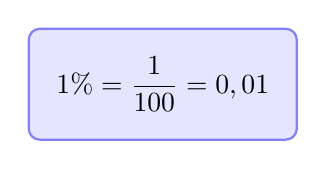
\begin{tikzpicture}
\node[rectangle, fill=blue!10, rounded corners, inner sep=10pt, draw=blue!50, thick] (box) {
$\displaystyle 1\% = \frac{1}{100} = 0,01$
};
\end{tikzpicture}

\subsection*{Representações}
\begin{itemize}
\item \textbf{Forma percentual}: 25\%
\item \textbf{Forma fracionária}: $\frac{25}{100} = \frac{1}{4}$
\item \textbf{Forma decimal}: 0,25
\end{itemize}

\section*{Fórmulas Importantes}

\subsection*{Cálculo da Porcentagem}

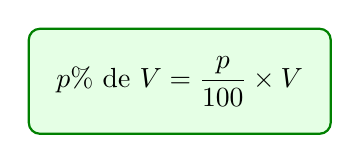
\begin{tikzpicture}
\node[rectangle, fill=green!10, rounded corners, inner sep=10pt, draw=green!50!black, thick] (box) {
$\displaystyle p\% \text{ de } V = \frac{p}{100} \times V$
};
\end{tikzpicture}

\textbf{Onde:}
\begin{itemize}
\item $p$ = taxa percentual
\item $V$ = valor total
\end{itemize}

\subsection*{Exemplo 1:}
Calcular 20\% de 300:
\[
20\% \text{ de } 300 = \frac{20}{100} \times 300 = 0,20 \times 300 = 60
\]

\subsection*{Exemplo 2:}
Uma camisa custa R\$ 80,00 com desconto de 15\%. Qual o valor do desconto?
\[
15\% \text{ de } 80 = \frac{15}{100} \times 80 = 0,15 \times 80 = 12
\]
Desconto = \textcolor{blue}{R\$ 12,00}

\subsection*{Cálculo da Taxa Percentual}

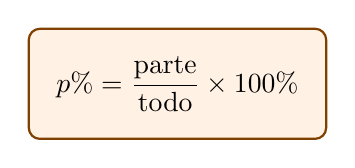
\begin{tikzpicture}
\node[rectangle, fill=orange!10, rounded corners, inner sep=10pt, draw=orange!50!black, thick] (box) {
$\displaystyle p\% = \frac{\text{parte}}{\text{todo}} \times 100\%$
};
\end{tikzpicture}

\subsection*{Exemplo 3:}
Em uma sala com 40 alunos, 10 foram aprovados. Qual a porcentagem de aprovação?
\[
p\% = \frac{10}{40} \times 100\% = 0,25 \times 100\% = 25\%
\]

\subsection*{Cálculo do Valor Total}

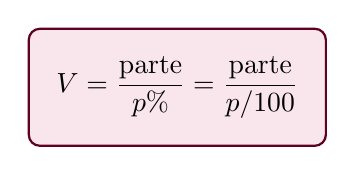
\begin{tikzpicture}
\node[rectangle, fill=purple!10, rounded corners, inner sep=10pt, draw=purple!50!black, thick] (box) {
$\displaystyle V = \frac{\text{parte}}{p\%} = \frac{\text{parte}}{p/100}$
};
\end{tikzpicture}

\subsection*{Exemplo 4:}
Se 15\% de um número é 45, qual é o número?
\[
V = \frac{45}{0,15} = 300
\]

\section*{Aumento e Desconto Percentual}

\subsection*{Aumento}
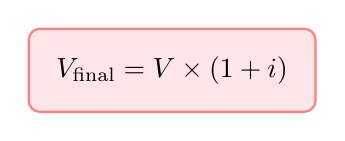
\begin{tikzpicture}
\node[rectangle, fill=red!10, rounded corners, inner sep=10pt, draw=red!50, thick] (box) {
$\displaystyle V_{\text{final}} = V \times (1 + i)$
};
\end{tikzpicture}

\subsection*{Desconto}
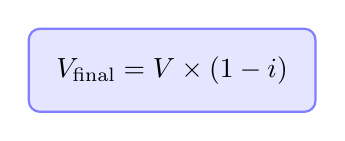
\begin{tikzpicture}
\node[rectangle, fill=blue!10, rounded corners, inner sep=10pt, draw=blue!50, thick] (box) {
$\displaystyle V_{\text{final}} = V \times (1 - i)$
};
\end{tikzpicture}

\textbf{Onde:} $i$ = taxa percentual (em decimal)

\subsection*{Exemplo 5 - Aumento:}
Um produto de R\$ 200,00 sofre aumento de 10\%:
\[
V_{\text{final}} = 200 \times (1 + 0,10) = 200 \times 1,10 = 220
\]

\subsection*{Exemplo 6 - Desconto:}
Uma televisão de R\$ 1200,00 com desconto de 15\%:
\[
V_{\text{final}} = 1200 \times (1 - 0,15) = 1200 \times 0,85 = 1020
\]

\section*{Porcentagem Sucessiva}

Dois aumentos sucessivos de 10\% equivalem a:
\[
(1 + 0,10) \times (1 + 0,10) = 1,10 \times 1,10 = 1,21
\]
\textbf{Taxa única:} 21\%

\section*{Exercícios Básicos}

\begin{enumerate}[leftmargin=*]

\item Converta para forma decimal:
\begin{enumerate}[label=\alph*)]
\item 15\%
\item 8\%
\item 120\%
\item 0,5\%
\end{enumerate}

\item Converta para porcentagem:
\begin{enumerate}[label=\alph*)]
\item 0,25
\item 0,75
\item 1,5
\item 0,02
\end{enumerate}

\item Calcule:
\begin{enumerate}[label=\alph*)]
\item 30\% de 200
\item 12\% de 500
\item 25\% de 80
\item 8\% de 150
\end{enumerate}

\item Complete a tabela:
\begin{center}
\begin{tabular}{|c|c|c|}
\hline
\textbf{Total} & \textbf{Porcentagem} & \textbf{Valor} \\
\hline
300 & 20\% & \\
500 & 15\% & \\
200 & & 50 \\
400 & & 32 \\
\hline
\end{tabular}
\end{center}

\item Problemas de desconto:
\begin{enumerate}[label=\alph*)]
\item Uma calça custa R\$ 120,00. Na liquidação, tem 20\% de desconto. Qual o preço final?
\item Um celular de R\$ 800,00 está com 12\% de desconto. Quanto pagarei?
\end{enumerate}

\item Problemas de aumento:
\begin{enumerate}[label=\alph*)]
\item O aluguel de R\$ 600,00 aumentou 8\%. Qual o novo valor?
\item Um funcionário ganhava R\$ 1500,00 e recebeu 5\% de aumento. Qual seu novo salário?
\end{enumerate}

\item Calcule a taxa percentual:
\begin{enumerate}[label=\alph*)]
\item 30 acertos em 40 questões
\item 12 meninas em uma turma de 30 alunos
\item 45 gols em 60 jogos
\item R\$ 18,00 de desconto em uma compra de R\$ 120,00
\end{enumerate}

\item Problemas com porcentagem:
\begin{enumerate}[label=\alph*)]
\item Em uma prova de 50 questões, acertei 40. Qual foi meu percentual de acerto?
\item Uma loja vendeu 180 de 200 produtos. Qual a porcentagem vendida?
\item Dos 500 alunos de uma escola, 125 usam óculos. Qual a porcentagem?
\end{enumerate}

\end{enumerate}

\section*{Exercícios Intermediários}

\begin{enumerate}[leftmargin=*, start=9]

\item Aumentos e descontos sucessivos:
\begin{enumerate}[label=\alph*)]
\item Um produto sofre dois aumentos sucessivos de 10\%. Qual o aumento total?
\item Um produto com desconto de 20\% e depois outro desconto de 10\%. Qual o desconto total?
\end{enumerate}

\item Calcule o valor original:
\begin{enumerate}[label=\alph*)]
\item Após um aumento de 15\%, um produto passou a custar R\$ 230,00. Qual era o preço original?
\item Com desconto de 25\%, paguei R\$ 150,00 em um tênis. Qual era o preço original?
\end{enumerate}

\item Comparação percentual:
\begin{enumerate}[label=\alph*)]
\item João tinha R\$ 200,00 e Pedro R\$ 150,00. Quanto João tem a mais que Pedro em porcentagem?
\item Em uma turma, 15 alunos gostam de Matemática e 25 de Português. Quantos porcento a mais gostam de Português?
\end{enumerate}

\item Situações do dia a dia:
\begin{enumerate}[label=\alph*)]
\item Um investimento de R\$ 1000,00 rendeu 12\% em um ano. Qual o montante?
\item Uma população de 5000 habitantes cresceu 8\% em um ano. Qual a nova população?
\item Um carro de R\$ 40.000,00 desvalorizou 15\% em um ano. Qual seu novo valor?
\end{enumerate}

\item Interpretação de gráfico (pizza):
\begin{center}
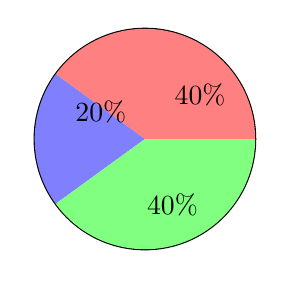
\begin{tikzpicture}[scale=0.7]
\draw[thick] (0,0) circle (2cm);
\fill[red!50] (0,0) -- (0:2cm) arc (0:144:2cm) -- cycle;
\fill[blue!50] (0,0) -- (144:2cm) arc (144:216:2cm) -- cycle;
\fill[green!50] (0,0) -- (216:2cm) arc (216:360:2cm) -- cycle;
\node at (1,0.8) {40\%};
\node at (-0.8,0.5) {20\%};
\node at (0.5,-1.2) {40\%};
\end{tikzpicture}
\end{center}
Se o total de pessoas é 500, quantas correspondem a cada setor?

\item Porcentagem de porcentagem:
\begin{enumerate}[label=\alph*)]
\item 20\% de 30\% de 500
\item 50\% de 10\% de 1000
\end{enumerate}

\end{enumerate}

\section*{Exercícios Avançados}

\begin{enumerate}[leftmargin=*, start=15]

\item Um produto teve dois aumentos sucessivos: 10\% e depois 15\%. Qual foi o aumento total?

\item Uma loja oferece dois descontos sucessivos de 10\% e 5\%. Qual o desconto único equivalente?

\item Em uma sala, 60\% dos alunos são mulheres. Se 25\% das mulheres usam óculos, qual a porcentagem de mulheres que usam óculos em relação ao total?

\item Uma mercadoria custava R\$ 200,00. Sofreu um aumento de 20\% e depois um desconto de 20\%. Qual o preço final?

\item Em uma pesquisa, 40\% preferem o produto A, 35\% o produto B e o restante o produto C. Se 50 pessoas preferem o produto C, qual o total de entrevistados?

\item Um salário de R\$ 2000,00 teve reajuste de 8\% e depois outro de 5\%. Qual o salário final?

\item Calcule o valor inicial:
\begin{enumerate}[label=\alph*)]
\item Após dois aumentos sucessivos de 10\%, o valor ficou R\$ 484,00
\item Após dois descontos sucessivos de 20\%, o valor ficou R\$ 320,00
\end{enumerate}

\item Represente graficamente:
\begin{enumerate}[label=\alph*)]
\item Uma pesquisa com 200 pessoas sobre preferência de sorvete: 50\% chocolate, 30\% morango, 20\% baunilha
\end{enumerate}

\end{enumerate}

\section*{Dicas para Resolver}

\begin{itemize}
\item \textbf{Transformação}: Para calcular, sempre transforme \% em decimal (divida por 100)
\item \textbf{Parte/Todo}: Para encontrar a taxa, use $\frac{\text{parte}}{\text{todo}} \times 100\%$
\item \textbf{Aumento}: Multiplique por $(1 + i)$
\item \textbf{Desconto}: Multiplique por $(1 - i)$
\item \textbf{Aumentos sucessivos}: Multiplique os fatores $(1 + i_1) \times (1 + i_2) \times \ldots$
\item \textbf{Descontos sucessivos}: Multiplique os fatores $(1 - i_1) \times (1 - i_2) \times \ldots$
\end{itemize}

\section*{Macete: Regra de Três}

Porcentagem é uma regra de três direta:
\[
\begin{array}{c|c}
100\% & \text{Total} \\
p\% & \text{Valor desejado}
\end{array}
\]
\[
\text{Valor desejado} = \frac{p \times \text{Total}}{100}
\]

\section*{Aplicações Práticas}

\begin{itemize}
\item \textbf{Finanças}: Juros, descontos, investimentos
\item \textbf{Vendas}: Promoções, comissões, impostos
\item \textbf{Estatística}: Pesquisas, índices, taxas
\item \textbf{Ciências}: Concentrações, proporções
\item \textbf{Dia a dia}: Gorjetas, descontos, aumento salarial
\end{itemize}

\section*{Tabela de Conversão Rápida}

\begin{center}
\begin{tabular}{|c|c|c|}
\hline
\textbf{Fração} & \textbf{Decimal} & \textbf{Porcentagem} \\
\hline
$\frac{1}{2}$ & 0,5 & 50\% \\
$\frac{1}{4}$ & 0,25 & 25\% \\
$\frac{3}{4}$ & 0,75 & 75\% \\
$\frac{1}{5}$ & 0,2 & 20\% \\
$\frac{1}{10}$ & 0,1 & 10\% \\
\hline
\end{tabular}
\end{center}

\end{multicols}

\end{document}
